\subsection{Esercizi tecnici}
\begin{questions}
	\question
	\begin{minipage}[b]{0.6\textwidth}
		In riferimento allo spazio 3D a fianco (lato 
quadrato unità di misura=10 cm) determinare per il 
triangolo isoscele:
\begin{itemize}
	\item  le dimensioni dei lati AB, BC e AC
	\item le dimensioni degli angoli interni $\alpha$, $\beta$ e $\gamma$
	\item l'Area ed il Perimetro
\end{itemize}
	\end{minipage}
	\hfill
\raisebox{-1\baselineskip}{
		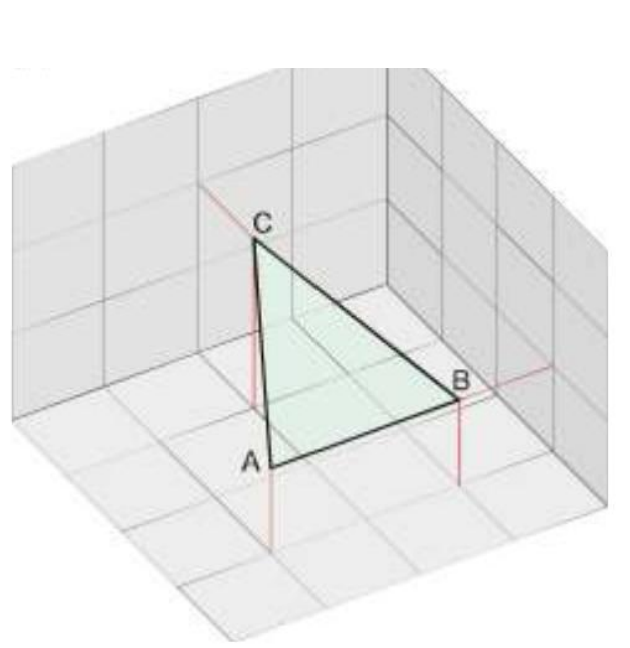
\includegraphics[width=0.3\textwidth]{3d-0-1}}

 
		\question
		\begin{minipage}[b]{0.6\textwidth}
			In riferimento allo spazio 3D a fianco (lato 
	quadrato unità di misura=10 cm) determinare per il 
	triangolo isoscele:
	\begin{itemize}
		\item  le dimensioni dei lati AB, BC e AC
		\item le dimensioni degli angoli interni $\alpha$, $\beta$ e $\gamma$
		\item l'Area ed il Perimetro
	\end{itemize}
		\end{minipage}
		\begin{minipage}{0.3\textwidth}
			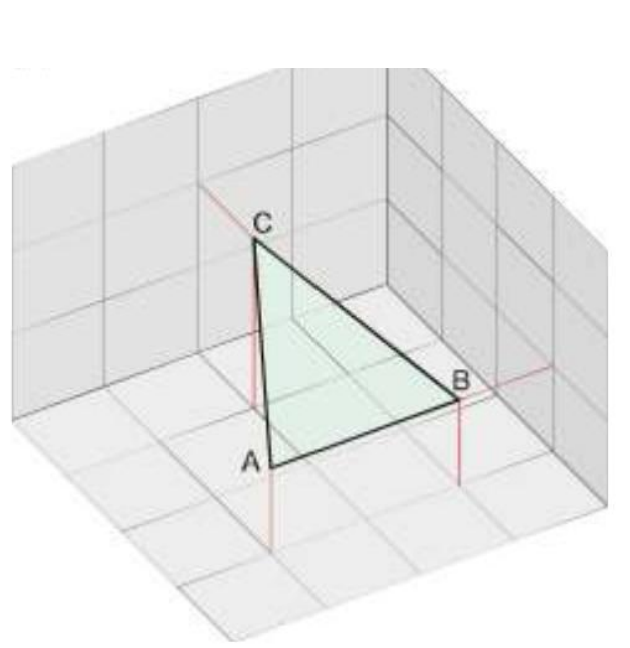
\includegraphics[scale=0.7]{3d-0-1}
		\end{minipage}

		\question
		\begin{minipage}[b]{0.6\textwidth}
			In riferimento allo spazio 3D a fianco (lato 
	quadrato unità di misura=10 cm) determinare per il 
	triangolo isoscele:
	\begin{itemize}
		\item  le dimensioni dei lati AB, BC e AC
		\item le dimensioni degli angoli interni $\alpha$, $\beta$ e $\gamma$
		\item l'Area ed il Perimetro
	\end{itemize}
		\end{minipage}
		\begin{minipage}{0.3\textwidth}
			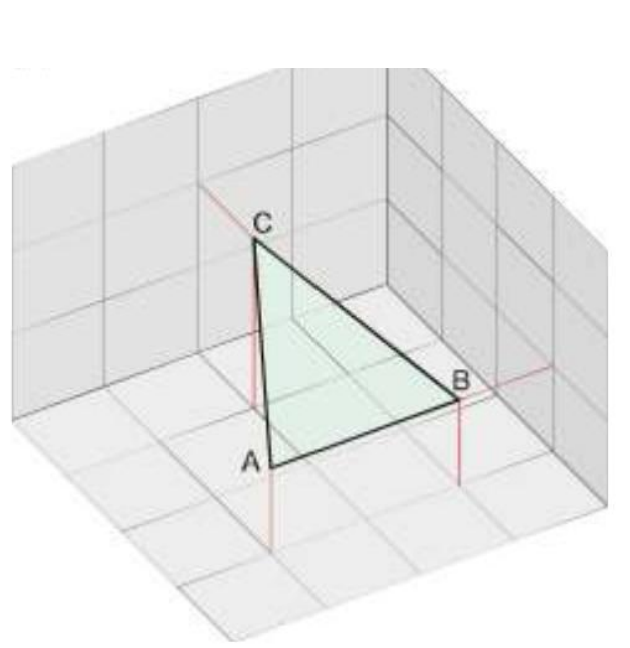
\includegraphics[scale=0.7]{3d-0-1}
		\end{minipage}
\end{questions}